\newpage
\section{恒星结构与演化}
恒星是星系的基本单元. 要了解星系和宇宙, 必须首先了解恒星的形成与演化. 恒星的结构与演化理论是20世纪天体物理最具标志性的重要成果之一! 
\subsection{恒星的形成与结构}

\subsubsection{原初恒星的形成}
原初恒星形成于分子云, 其塌缩形成原恒星. 

假设分子云的密度为 $\rho$, 温度为$T$, 考虑一个半径为$R$的球体, 其由于引力不稳定性导致塌缩的条件为总能量小于0, 即 $E+K<0$, $E$为该球体的势能, $K$为动能. 

假设密度均匀, 球体内总质量 $M=\frac{4\pi}{3}\rho R^3$,且 $\rho=n_H m_H$, $n_H$ 为等效氢原子数密度, $m_H$ 为氢原子质量. 

该球体的总势能、总动能 分别为
\begin{align*}
    E&=\frac{3}{5}\frac{GM^2}{R}\\
    K&=N\frac{3}{2}kT=\frac{M}{m_H}\frac{3}{2}kT
\end{align*}
代入可得分子云塌缩的临界半径
\begin{align*}
    R_J=\sqrt{a_1\frac{T}{n_H}}
\end{align*}
这里 $a_1=15k/(8\pi G m_H^2) \approx 4.4 \times 10^{40}(1/mK)$, $R_J$ 也叫金斯半径, 对应的金斯质量. 
\begin{align*}
    M_J=a_2T^{1.5}n_H^{-0.5}
\end{align*}
$a_2=6.5\times 10^{34}(kg/(m^{1.5}K^{1.5}))$, 引入太阳质量 $1M_{\odot}=2\times 10^{30}kg$, $M_J\approx 30\sqrt{\frac{T^3}{n_H}}M_{\odot }$ 

\begin{itemize}
    \item 对于典型分子云温度 $30K$, 密度$10^3/cm^3$, 可得 $R_J=1.18 pc, M_J\approx 170 M_{\odot}$
    \item 对于典型分子云温度 $30K$, 密度$10^4/cm^3$, 可得 $R_J=0.37 pc, M_J\approx 48 M_{\odot} $
    \item 中性氢云: $1/cm^3, T=100K, M_J \approx 30000 M_{\odot}$
    \item 暗分子云: $10^6/cm^3, T=10K, M_J \approx 1 M_{\odot}$
\end{itemize}
恒星更容易形成于分子云. 

金斯方程的另外一种推导 (向内的引力大于内部压力) 此略. 

金斯质量 $M_J=a_2T^{1.5}n_H^{-0.5}$ 对应于分子云可以自引力塌缩的最小质量.  可以知道, 对于冷气体或者密度高 , 其金斯质量越小, 越容易在不稳定情况下发生塌缩.  

\subsubsection{自由下落时标 (free fall time)}
对于一块半径为$R$的塌缩云, 其塌缩所需时间. 

自由下落引力加速度 $a=\frac{GM}{R^2}$, 自由下落距离 $R\approx 0.5at^2$, 初始时 $M=\frac{4\pi}{3}\rho R^3$, 可得
\begin{align*}
    t_{ff}=\sqrt{\frac{3}{2\pi G\rho}}\approx 10^6 yr\sqrt{\frac{10^4cm^{-3}}{n}}
\end{align*}
可以看到塌缩时标 $t_ff$ 与质量无关, 只依赖于气体密度, 密度越大, 自由下落时标越短. 

对于 $n=2\times 10^3 cm^{-3}$, $t_{ff}\approx 2.24\times 10^6 yr$ 分子云典型塌缩时标为百万年. 


从金斯质量 $M_J$ 可以看出, 如果在分子云塌缩过程中, 云收缩而释放的引力能被辐射出去, 从而保持气体云温度不变, 则$M_J\approx \rho^{-0.5}$, 即塌缩过程中密度变高, 金斯质量变小, 因此气体云可以破碎成更小的分子云. 

\begin{figure}[!htb]
    \centering
    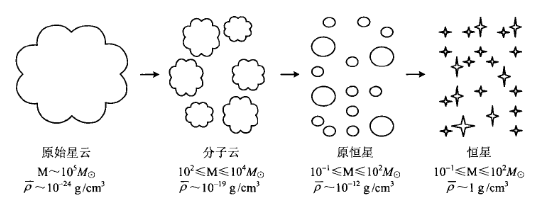
\includegraphics[width=0.479\textwidth]{GA3/原始星云的碎裂, 凝聚过程}
    \caption{原始星云的碎裂, 凝聚过程}
\end{figure}

\subsubsection{恒星的结构}
处于平衡态恒星满足的基本方程. 
\begin{enumerate}
    \item 质量方程
    球壳 $(r,\ r+\mathrm{d}r)$ 内物质 $\mathrm{d}m=4\pi r^2 \mathrm{d}r \rho$
    \begin{align*}
        \frac{\mathrm{d} m}{\mathrm{d} r}=4\pi r^2 \rho
    \end{align*}
    \item 流体静力学平衡:引力=压力
    
    球壳 $(r,\ r+\mathrm{d}r)$ 收到的压力 $\mathrm{d}P S=\mathrm{d}P 4\pi r^2$, 注意这里压力$P$包括气体压和辐射压, 受到的引力 $F=-\frac{G m(<r)}{r^2}\mathrm{d}m=-\frac{G m}{r^2} 4\pi r^2 \mathrm{d}r \rho$
    \begin{align*}
        \frac{\mathrm{d}P}{\mathrm{d}r}=-\frac{Gm}{r^2}\rho
    \end{align*}
    \item 能量平衡: 球壳向外流出的能量=球壳内产生的能量
    
    $\mathrm{d}L_r =\mathrm{d}m \varepsilon$, 这里$L_r$表示半径$r$处辐射的能量,  $\varepsilon$ 表示单位质量的产能率. 恒星内部产生能量的机制有
    \begin{enumerate}
        \item 热核反应释放能量$\varepsilon_n$
        \item 由于物质热状态发生改变而释放的能量 $\varepsilon_g$(内能和膨胀做功)
        \item 通过中微子辐射而损失能量$-\varepsilon_v$
    \end{enumerate}
    \begin{align*}
        \frac{\mathrm{d}L_r}{\mathrm{d}m}=\varepsilon_n+\varepsilon_g-\varepsilon_v
    \end{align*}
    \item 辐射转移方程
    \item 
    能量从恒星内部传送到外部, 主要有辐射, 对流和热传导三种输运方式, 一般来说辐射和对流占主导, 这里只考虑辐射传能方式. 
\end{enumerate}

\begin{figure}[!htb]
    \centering
    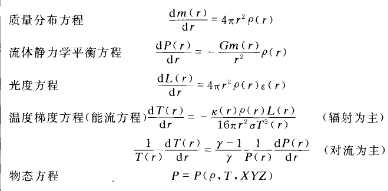
\includegraphics[width=0.479\textwidth]{GA3/恒星结构的基本方程}
    \caption{恒星结构的基本方程}
\end{figure}
这5个方程要确定5个未知量: $m, \rho, P, L, T,$ (它们都是$r$的函数), 该方程组是闭合的, 可以通过数值计算方法求解, 只是产能率, 吸收系数, 元素组成等需要事先给定. 

经过严格证明:平衡的恒星球体内部结构, 由它的化学成分和总质量唯一确定. 但恒星内部发生核燃烧后, 化学成分变化, 恒星结构随之变化. 求解上述方程非常复杂. 

\subsubsection{恒星结构方程的简单应用}
\begin{enumerate}
    \item 太阳中心压强和温度估计
    
    流体静力学平衡方程
    \begin{align*}
        \frac{\mathrm{d}P}{\mathrm{d}r}=-\frac{Gm}{r^2}\rho
    \end{align*}
    近似可得
    \begin{align*}
        \frac{P_c-P_0}{R}=\frac{GM}{R^2}\bar{\rho}
    \end{align*}
    代入 $M=\frac{4}{3}\pi R^3 \bar{\rho}$, 且在恒星表面 $P_0\approx 0$,  可得
    \begin{align*}
        P_c\approx \frac{GM^2}{4R^4}
    \end{align*}
    代入太阳质量和半径
    \begin{align*}
        P_c\approx 2.8\times 10^{15}\left( \frac{M}{M_{\odot}} \right)^2 \left( \frac{R_{\odot}}{R} \right)^4
    \end{align*}
    由此可看出, 太阳中心压强$\approx 10^{15} cgs \approx 10^{12}$大气压. 

    太阳中心温度, 由 $P_c\sim nkT$, 
    \begin{align*}
        T\approx 10^7 u \left( \frac{M}{M_{\odot}} \right) \left( \frac{R_{\odot}}{R} \right) \approx 10^7 K
    \end{align*}
    太阳中心温度1000万度. 

    \item 位力定理
    \begin{align*}
        \frac{\mathrm{d}P}{\mathrm{d}r}=-\frac{Gm}{r^2}\rho
    \end{align*}
    两边同时乘以$4\pi r^3 \mathrm{d}r$, 并积分可得
    \begin{align*}
        \int_0^R 4\pi r^3\ \mathrm{d}P=-\int_{0}^{M}\frac{Gm}{r}\ \mathrm{d}m
    \end{align*}
    左边分部积分, 变成
    \begin{align*}
        \int_0^R 4\pi r^3\ \mathrm{d}P=\left.(4\pi r^3 P)\right|_0^R - 3\int_0^R 4\pi r^2 P \ \mathrm{d}r
    \end{align*}
    注意到$r=R$时$P=0$ (恒星表面), 得到
    \begin{align*}
        3\int_0^R \frac{4\pi r^2 \rho}{\rho} P \ \mathrm{d}=3\int_{0}^{M}\frac{P}{\rho}\ \mathrm{d}m
    \end{align*}
    对于单原子理想气体, 对于单位质量气体, 其内能 
    \begin{align*}
        \varepsilon=\frac{3}{2}\frac{kT}{u m_p}
    \end{align*}
    利用
    \begin{align*}
        P=nkT=\frac{\rho}{u m_p}kT
    \end{align*}
    即
    \begin{align*}
        \frac{P}{\rho}=\frac{2}{3}\varepsilon
    \end{align*}
    \begin{align*}
        3\int_{0}^{M}\frac{P}{\rho}\ \mathrm{d}m=2\int_{0}^{M}\varepsilon\ \mathrm{d}m=2U
    \end{align*}
    这里$U$为恒星的总内能. 

    恒星总势能
    \begin{align*}
        V=-\int_{0}^{M}\frac{Gm}{r}\ \mathrm{d}m
    \end{align*}
    因此$2U+V=0$, 系统总能量$E=U+V=V/2$. 

    可以看到, 在恒星收缩过程中, 减少的势能中有一半能量转化为系统内能, 一半变成了辐射能, 释放到星际空间. 

    \item 恒星的脉动
    
    假设恒星内部发生扰动, 使得恒星失去流体静力学平衡, 则恒星将收缩或者膨胀, 在压强和引力之间建立新的平衡, 这称为恒星的脉动. 其典型周期为声波穿过恒星的时标. 
    \begin{align*}
        t\approx \frac{R}{V_s}
    \end{align*}
    声波速度$V_s$满足
    \begin{align*}
        V_s^2=\frac{\mathrm{d}P}{\mathrm{d}p}
    \end{align*}
    对于理想气体 $P=nkT$, 可得
    \begin{align*}
        V_s^2=\frac{kT}{um_H}
    \end{align*}
    由位力定理, 气体总内能
    \begin{align*}
        U=\frac{3}{2}NkT=\frac{3}{2}\frac{M}{um_H}kT\approx \frac{1}{2}\frac{GM^2}{R}
    \end{align*}
    略去相关系数, 可得
    \begin{align*}
        V_s^2=\frac{GM}{R}
    \end{align*}
    可以得到脉动周期
    \begin{align*}
        t\approx\sqrt{\frac{R^3}{GM}}\approx \rho^{-0.5}
    \end{align*}
    与自由下落时标接近. 

    典型时标: 
    \begin{itemize}
        \item 太阳, $R=6.9\times10^{10} cm, M=2\times10^{33} g$, 可得其周期为25分. 
        \item 巨星(造父变星), $R=10^2R_{\odot}$, 周期20天. 
        \item 白矮星: $R=0.1R_{\odot}, M\approx M_{\odot}$, 周期5秒. 
    \end{itemize}
    对于造父变星, 其恒星质量和表面温度无太大变化, 但是由于其具有不同的半径$R$, 可以看到$R$越大, 亮度$L\approx R^2T^4$越大, 周期越长, 因此存在周光关系. 

    \item 开尔文-亥姆霍兹时标
    
    认为恒星(太阳)的能源来自其引力收缩释放的引力能, 明显小于地球物种演化年龄, 恒星(太阳)的能源肯定不是来自其引力能, 而是来自核反应. 
    \item 爱因斯坦时标
    
    太阳的总能量
    \begin{align*}
        E=Mc^2
    \end{align*}
    为$1.8\times 10^{54} erg$, 因此太阳以目前光度可维持的时间$t_E \approx \frac{E}{L_{\odot}} \approx 1.4\times10^{13} $年. 从恒星演化理论, 我们知道太阳的寿命为$10^{10}$年. 因此可见太阳中质量转化为能量的效率$\sim 7\%$. 
    
    热核聚变只发生在恒星内部, 其质量为恒星总质量的$\sim 10\%$. 
\end{enumerate}

\subsubsection{赫罗图}
赫罗图 (HR Diagram: Hertzsprung-Russell Diagram): 表征恒星演化的途径. X-axis: 恒星表面温度, y-axis: 恒星亮度. 

\begin{figure}[!htb]
    \centering
    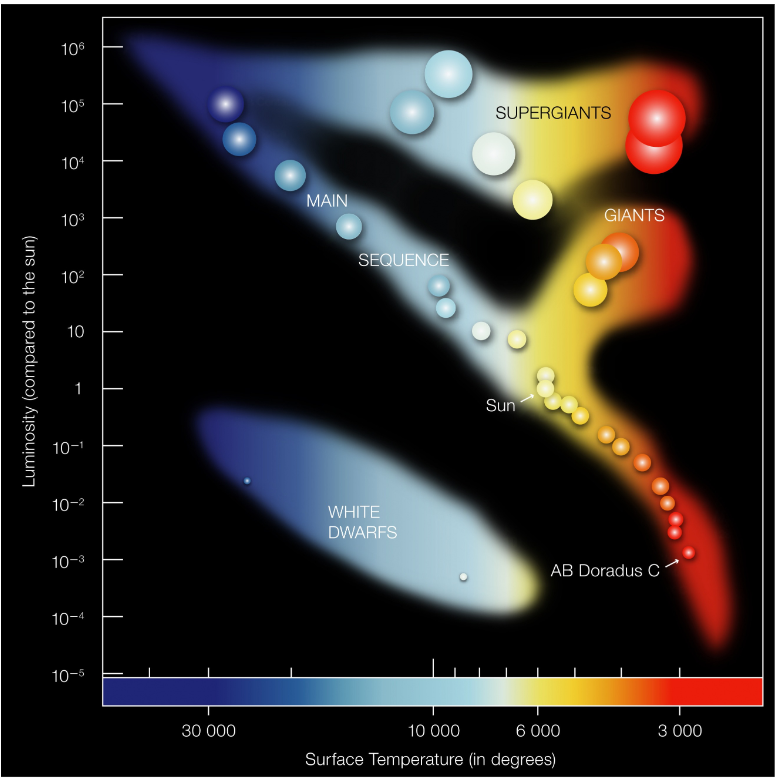
\includegraphics[width=0.309\textwidth]{GA3/赫罗图}
    \caption{赫罗图}
\end{figure}

\subsubsection{主序恒星}
恒星将在主序带渡过它一生的绝大部分时间

主序恒星的特征: 
\begin{enumerate}
    \item 恒星辐射近似为黑体谱: 温度为$T$, 半径 $R$的黑体, 由Stefan-Boltzmann law可得其光度$L=4\pi R^2 \sigma T^4$
    \item 光度-质量关系: 观测发现主序星具有$L\sim M^{3.5}$, 一个30太阳质量的恒星, 亮度为太阳的10万倍. 
    \item 半径-质量关系: $R\sim M^{0.8}$ (除了太阳以外, 恒星半径无法直接观测, 一般根据恒星$L$-$T$关系来得到, $T$从恒星光谱可得到)
    \item 主序恒星寿命: $t\sim \frac{E}{L}\sim \varepsilon \frac{M}{L} \sim M^{-2.5} $ (假设恒星总能量来自核反应, 质能方程$E\sim \varepsilon Mc^2$), 大质量恒星寿命短.     
\end{enumerate}

\subsection{元素核反应}
恒星的内部能源: 克服库伦势垒, 或通过量子隧穿效应, 发生的核聚变. 不同原子核反应需要的温度不同, 主要取决于恒星的总质量.   

恒星的初始物质组成主要为氢, 氦. 依赖于恒星质量(中心温度), 恒星内元素主要通过如下途径发生核反应: 
\begin{enumerate}
    \item 质子-质子链氢核聚变反应(Proton-Proton, PP链) 
    \item CNO循环
    \item 3-alpha反应
    \item 其他核反应
\end{enumerate}


\subsection{恒星的演化轨迹}
\subsubsection{褐矮星 (Brown dwarf)}

\begin{figure}[!htb]
    \centering
    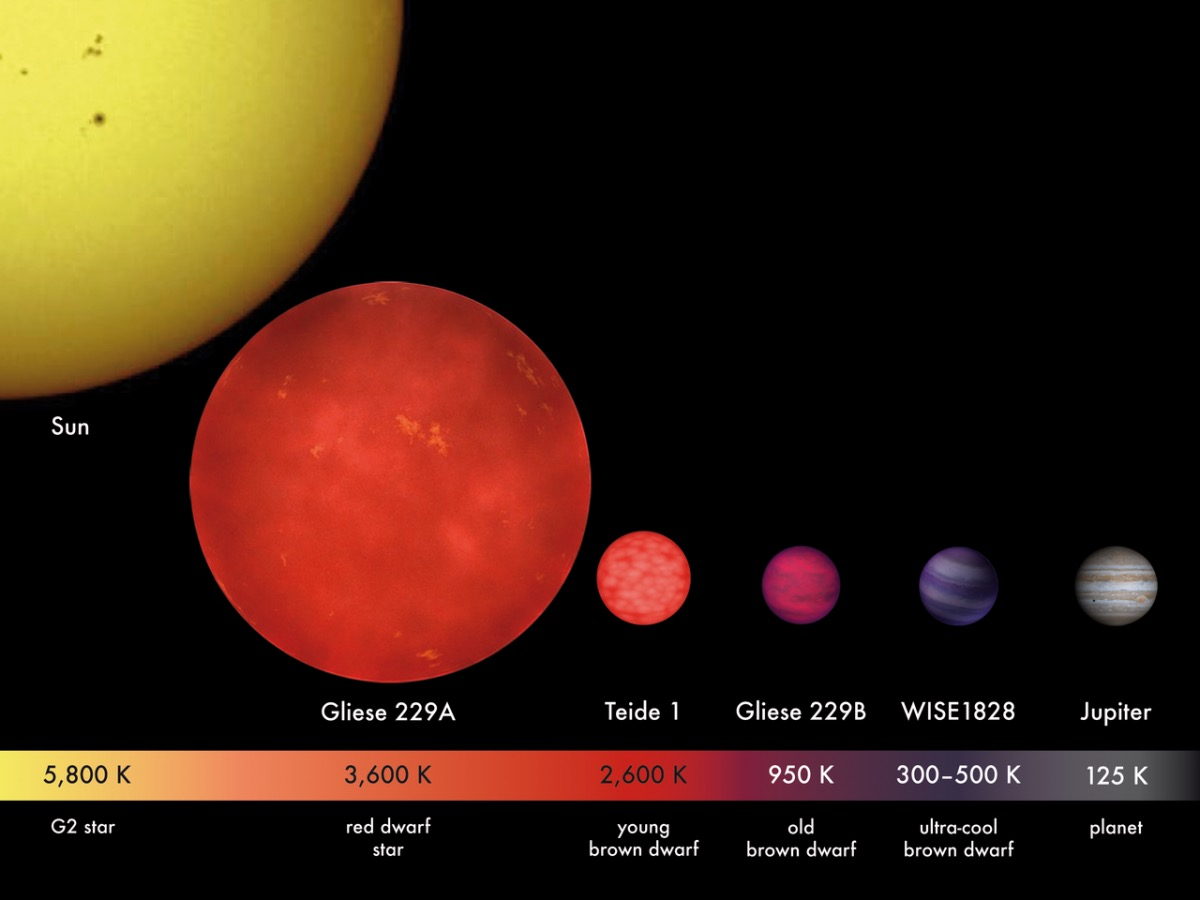
\includegraphics[width=0.309\textwidth]{GA3/褐矮星}
    \caption{褐矮星}
\end{figure}


质量小于$0.08M_{\odot}$的天体, 于其自身引力不足以使中心区域达到氢点火的温度, 因此不能靠核反应发光, 只能依靠气体热辐射发光. 这样的天体不能称为恒星, 有时称为失败的恒星. 在银河系中已经发现大量的褐矮星. 

褐矮星与行星在形成机制, 物质组成上存在本质区别. 

恒星在绝大部分时间处于主序上, 其停留时间取决于中心区域氢燃烧过程. 当氢燃烧完之后, 恒星离开主序, 在赫罗图上演化. 

\begin{figure}[!htb]
    \centering
    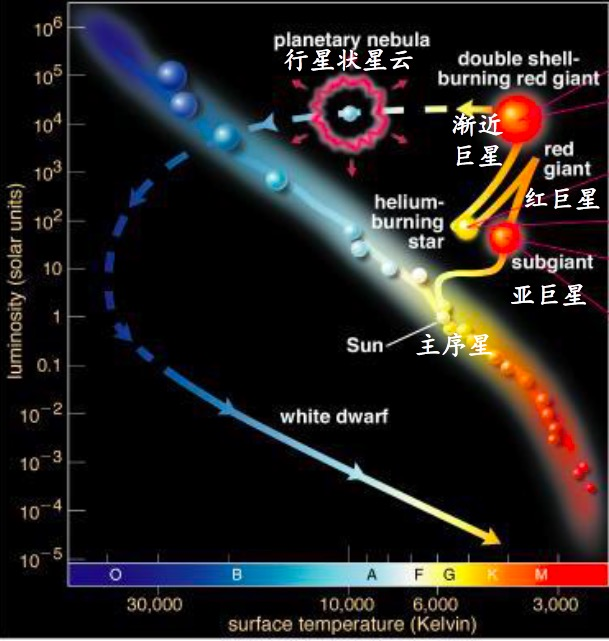
\includegraphics[width=0.309\textwidth]{GA3/恒星的演化}
    \caption{恒星的演化}
\end{figure}


\subsubsection{低质量恒星演化}
\begin{enumerate}\small
    \item 主序$\rightarrow$亚巨星: 低质量恒星, 当其中心氢燃烧完之后, 将形成一个氦核和含有氢的外层. 此时中心区域温度不够高, 不足以使氦发生聚变, 因此中心为一个“冷”的核. 在冷氦核的表面氢继续燃烧, 维持恒星辐射的大部分能量. 当氢壳层燃烧生成氦, 导致氦核质量增加开始引力收缩, 释放引力能注入到氢外层, 导致外层膨胀, 恒星半径变大, 温度降低. 在赫罗图上向右上方移动, 形成亚巨星. 
    \item 红巨星: 由于外层气体对光子的阻挡作用, 恒星表面温度下降到一定程度后保持不变, 但是恒星半径继续增加, 亚巨星在赫罗图上几乎垂直向上, 形成红巨星. 
    \item 氦闪 (未被观测, 仅理论推测): 红巨星之后, 随着中心区域的质量不断增加核引力收缩, 中心氦区温度继续上升, 当温度超过 $10^8$K以后, 氦开始燃烧, 发生3-alpha反应, 生成${}^12$ C. 核区温度升高, 中心发生绝热膨胀, 但是由于电子简并压力不减小, 核反应加速进行, 形成所谓的氦闪. 该过程时间很短, 大概几秒-几分钟. 
    \item 氦燃烧稳定阶段(水平分支)): 氦闪导致核区温度升高, 密度不变, 核区内电子从简并变为非简并, 此时核区膨胀, 吸热, 光度降低, 恒星在赫罗图上向左下移动, 进入稳定的氦燃烧阶段 (3-alpha反应). 同时也会生成部分氧. 
    \subitem 氦核周围是氢壳层燃烧. 该状态称为水平分支, 其在赫罗图上的具体位置与恒星初始质量, 红巨星阶段的质量损失有关. 
    \item 渐进巨星分支(Asymptotic Giant Brant: AGB): 当核心的氦耗尽, 中心变成碳-氧核, 核心再次收缩, 导致外层氦燃烧, 其再之外为氢燃烧. 这是恒星处于双壳层燃烧阶段, 恒星光度增加, 再次到红巨星(红超巨星). 
    \item 行星状星云(Planetary Nebula)在红超巨星阶段, 外层物质损失非常快, 壳层燃烧物质迅速靠近表面而消失,  大量物质被抛射到恒星际空间, 导致恒星在赫罗图上向左移动, 变成行星状星云. 在星云中心, 则是一颗孤零的白矮星. 
    
    白矮星: $M_{\odot}, 0.01R_{\odot}$
\end{enumerate}

\subsubsection{中质量恒星演化}
$2.3M_{\odot}<M<8M_{\odot}$, 中等质量的恒星演化轨迹与小质量恒星差不多, 但是呈现一些不同的特点
\begin{enumerate}\small
    \item 主序 --- 红巨星: 演化到红巨星阶段时间非常短, $\sim 3*10^6$ 年, 在赫罗图留下空隙区. 
    \item 激发脉动: 在外壳层中的氢、氦电离区形成激发脉动, 在赫罗图上左右来回摆动, 中
    间穿过造父脉动带区域, 形成造父变星. 
    \item AGB阶段: 巨大的星风, 并有大量中微子产生
    \item 最终演化
    \begin{itemize}
        \item 超新星 $\sim 8M_{\odot}$
        \item 行星状星云+碳氧白矮星 $2.3\sim 6M_{\odot}$
    \end{itemize}
\end{enumerate}

\subsubsection{大质量恒星演化}
$>8M_{\odot}$, 恒星内部温度更高, 导致其其演化时标非常快, 并有如下主要特点:
\begin{enumerate}\small
    \item 内部发生更多核反应: 生成C , O, Na, Mg, Si, P, S等, 最后形成铁核
    \item 内部强烈对流和更强物质外流:  重元素从恒星内部输运到恒星表面, 并经由强烈星风抛射到恒星际空间, 甚至恒星形成区之外
    \item 最终演化:  铁核非常不稳定, 很容易形成超新星
    \begin{itemize}
        \item 中子星 $8\sim 30M_{\odot}$
        \item 黑洞 $>30 M_{\odot}$
    \end{itemize}
\end{enumerate}


\subsubsection{小结}
不同质量恒星的演化:
\begin{enumerate}\small
    \item 都会经历光度上升阶段
    \item 大质量恒星演化快, 并且很快死亡
    \item 小质量恒星在主序的生存时间大于宇宙年龄
\end{enumerate}

% 单个恒星的光度演化

% \begin{figure}[!htb]
%     \centering
%     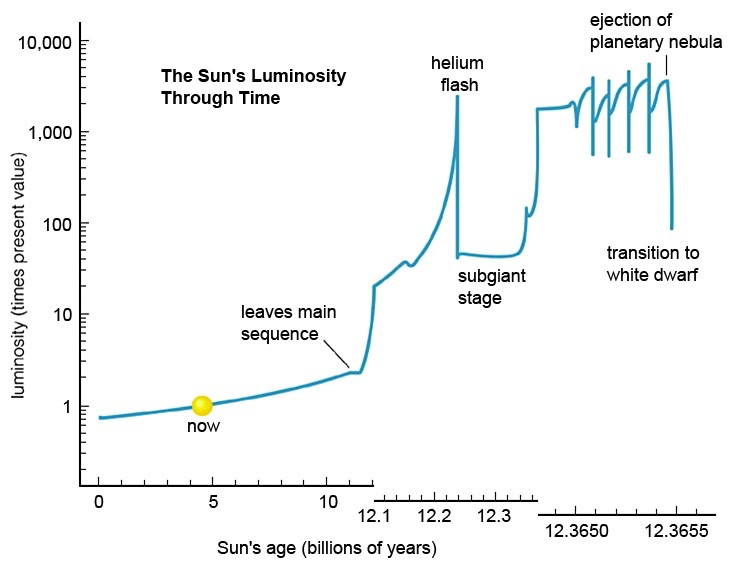
\includegraphics[width=0.309\textwidth]{GA3/单个恒星的光度演化}
%     \caption{单个恒星的光度演化}
% \end{figure}


\subsubsection{等年龄线(Isochrone)}
指的具有同样年龄、同样金属丰度、但不同质量的恒星在赫罗图上的分布. 对于球状星团, 其中恒星具有相同的年龄和金属丰度, 因此在HR图上的分布可以很好的用Isochrone来描述, 并可以得到星团的年龄. 

\begin{figure}[!htb]
    \centering
    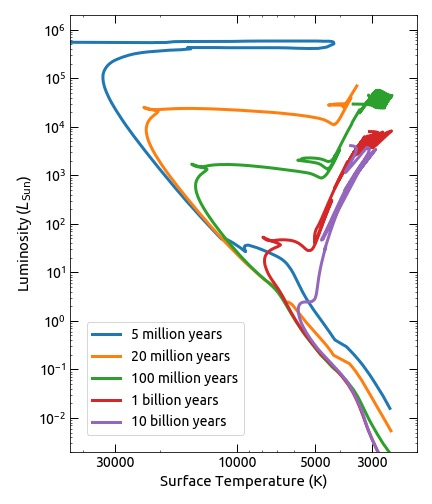
\includegraphics[width=0.309\textwidth]{GA3/等年龄线}
    \caption{等年龄线}
\end{figure}
\begin{itemize}
    \item 转折点---确定星族年龄
    \item 水平分支---确定距离
\end{itemize}

\subsubsection{恒星遗迹质量与初始质量关系}
恒星在演化过程中将通过如下途径损失质量, 但是损失量非常不确定, 强烈依赖于恒星原初化学成分:
\begin{itemize}\small
    \item 星风: 大质量恒星在演化过程中通过星风损失部分质量, 剩下白矮星
    \item 超新星爆炸: 爆炸将恒星外包层物质全部抛向恒星际空间, 留下黑洞或者中子星
\end{itemize}

对于某个星族, 总的遗迹质量依赖于恒星初始质量分布平均来说, 恒星将50\% 左右的物质返还到恒星际介质中(冷气体+热气体)

\begin{figure}[!htb]
    \centering
    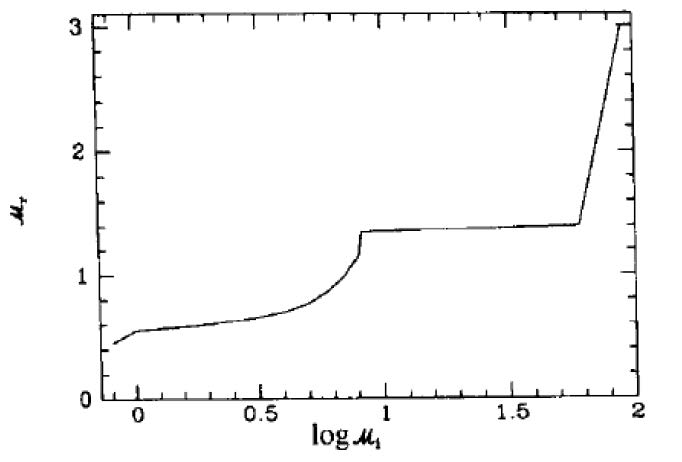
\includegraphics[width=0.309\textwidth]{GA3/恒星遗迹质量与初始质量关系}
    \caption{恒星遗迹质量与初始质量关系}
\end{figure}


\subsubsection{白矮星质量上限 (钱德拉塞卡极限)}
在中等质量恒星演化后期, 氦氧核燃烧结束, 由于失去核反应提供的热能和辐射压, 核区开始收缩, 核区密度变高, 当密度足够高时, 电子变为简并且处于相对论状态(其速度接近光速), 此时电子的压强与密度之间存在如下关系: 
\begin{align*}
    P\sim K(\rho/\mu_e)^{4/3},\ K=1.23*10^{10}
\end{align*}
利用之前的流体静力学平衡公式
\begin{align*}
    \frac{dP}{dR}=G\frac{M}{R^2}\rho
\end{align*}
\begin{itemize}
    \item 左边为压强项
    \begin{align*}
        \sim \frac{P}{R}\sim \frac{K(\rho/\mu_e)^{4/3}}{R} \sim \frac{KM^{4/3}}{R^5}
    \end{align*}
    \item 右边为引力项
    \begin{align*}
        \sim G\frac{M}{R^2}\rho \sim \frac{GM^2}{R^5}
    \end{align*}
\end{itemize}
可以看到随着质量增加, 引力比压强增加更快, 因此存在一个特征质量$M_{ch}$, 超过该质量后白矮星不能稳定(变成中子星或者黑洞). 

从上式可得白矮星的质量上限为
\begin{align*}
    KM^{4/3}\sim GM^2
\end{align*}
代入相关系数可得$M_{ch}\approx 1.4M_{\odot}$. 

\subsubsection{双星系统}
对于恒星质量分别为$m_1, m_2$ 的双星系统, 其满足开普勒第三定律
\begin{align*}
    G(m_1+m_2)P^2=4\pi^2 a^3
\end{align*}
$P$为旋转周期, $a$为相对运动轨道的半轴长. 

\small
因此, 只要测量到双星系统的旋转周期, 相对轨道的半长轴, 可以确定系统总质量. 如果假设双星系统的恒星亮度与质量成正比(对于质量相差不大的主序星系统, 该假设一般成立), 可以通过双星的光度比例分别测量出$m_1, m_2$. 
\normalsize

由于双星系统在围绕彼此旋转, 因此系统中恒星的星风会受到来自伴星的引力, 导致星风被伴星吸积, 发生物质交换, 从而影响恒星的演化. 在旋转双星系统中存在一个特殊的区域, 称为洛希等势面. 

\small
通过计算可以得到其等势面如图所示, 其中存在系列拉格朗日点, 在该点处, 一个受力粒子可以相对于两恒星保持静止. 通过拉格朗日点的等势面为临界等势面. 

\begin{figure}[!htb]
    \centering
    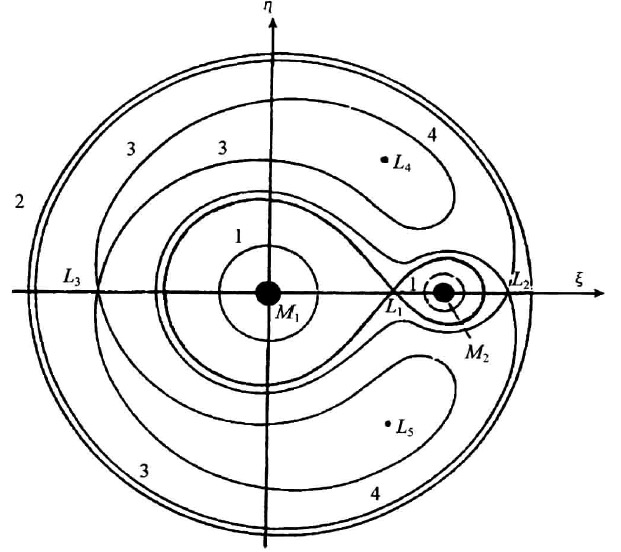
\includegraphics[width=0.239\textwidth]{GA3/等势面}
    \caption{等势面}
\end{figure}


通过L1的等势面具有特别的意义, 它包含的体积为洛希临界体积. 当恒星大气处于洛希体积内, 可以认为其受到另一个恒星的引力较小, 一旦达到洛希等势面, 恒星大气将发生交换, 从一个恒星到达另一个恒星.
\normalsize 

对于红巨星, 其物质充满洛希面以后, 将会流向体积较小的伴星(如白矮星), 一旦吸积物质后质量超过钱德拉塞卡极限, 白矮星将发生爆炸, 形成超新星. 

\begin{figure}[!htb]
    \centering
    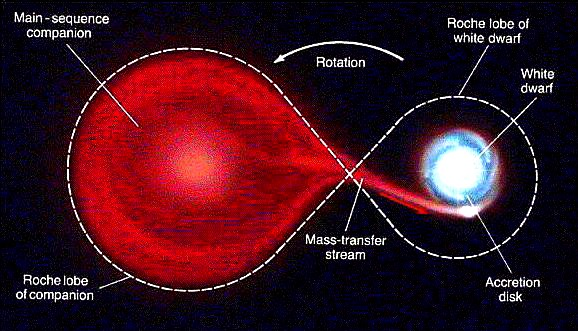
\includegraphics[width=0.309\textwidth]{GA3/洛希等势面}
    \caption{洛希等势面}
\end{figure}


\subsubsection{超新星}
超新星是一类独特而有常见的天文现象, 是恒星演化到晚期的最剧烈活动, 其爆发释放的能量可达 $10^{47\sim 53}$ erg, 亮度甚至超过整个星系. 

分类: 
\begin{enumerate}\small
    \item II型超新星
    \subitem 光谱中含有明显的氢吸收线, 大质量恒星的产物-中子星, 爆发率取决于星系的瞬时恒星形成率. 
    \subitem 爆发过程将重元素抛向恒星际空间. 
    \subitem 常见于恒星形成星系. 
    \item I型超新星
    \subitem 光谱中没有氢吸收线
    \subitem Ia: 没有氢氦线, 有硅吸收线, 常见种类型星系. 中等质量恒星的-白矮星, 爆发率非常不确定
    \subitem Ib: 有强的氦吸收线
    \subitem Ic: 几乎没有明显的吸收线
\end{enumerate}
Ib, Ic可能是大质量恒星外包层剥离后塌缩的超新星, 常见的超新星主要是Type-II and Type-Ia. 

\subsubsection{恒星初始质量函数 (IMF)}
IMF描述的是在星系中新生成的一批恒星中, 不同质量恒星之间的数目分布
\begin{align*}
    dN=N_0 * \xi (M)dM
\end{align*}
$N_0$ 表示新生成单位太阳质量恒星
的总数目, $\xi(M)$满足如下归一化条件
\begin{align*}
    M_{\odot}=\int M*\xi(M)dM
\end{align*}

Salpeter 1955年提出银河系的IMF具有一个简单的形式
\begin{align*}
    \xi(M)=M^{-\alpha}
\end{align*}
对所有$M$, $\alpha=2.5$(需在低质量处截断, 否则质量发散). 

后来的观测发现, IMF可以有其他形式, 并且随着环境和时间演化. 

实际上测量银河系的IMF也很困难. 有如下2个主要原因: 
\begin{enumerate}\small
    \item 演化和光度效应: 大质量恒星演化快, 并且大质量恒星处于恒星形成区, 有严重的尘埃遮挡效应. 小质量恒星($<1M_{\odot}$ )由于光度低, 很难完备测量. 
    \item 环境效应: 恒星盘、核球区等不同区域内IMF也不一样
\end{enumerate}
河外星系无法直接测量其单个恒星, 只能利用模型拟合. 